\documentclass{book}

\usepackage[]{graphicx}

\title{Design Document}
\author{Jens Henninger \and Daniel Maier \and Paul Fink \and Florian Jennewein}
\date{\today}


\begin{document}
\frontmatter
\maketitle
\tableofcontents
\mainmatter
\part{Architectural Design}

\chapter{Introduction}
This architectural document describes the architecture of the desired system "Sojabohne" from different perspectives and in different levels of detail. All references to requirements are based on the system requirements of our requirements-document from 26.11.2015\footnote{https://moodle.uni-mainz.de/pluginfile.php/33185/assignsubmission\_file/submission\_files/8942/Abgabe\_Review\_Document.tar.gz}.
\chapter{External Layer}
Because there is no connection between our system and other ones, Sojabohne is set in a standalone-context(cf.Figure 2.1). \\\\\\\\
\begin{figure}[h]
\centering
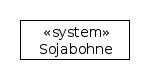
\includegraphics[width=3cm]{Context_Model.jpg}
\caption{Our system in standalone context :)}
\label{Fig. 1}
\end{figure}
\chapter{Structural Layer}
\chapter{Used Patterns}
\chapter{Interaction Layer}
The following section attends to the interaction between the different aleready mentioned system components in different scenarios. The main task is the visualization of the data exchange with sequence-diagrams; without an exact definition of the called methods.
 
\end{document}

%%% Local Variables:
%%% mode: latex
%%% TeX-master: t
%%% End:
